\section{Zeichnen mit TikZ}
\label{sec:tikz}

TikZ (ist kein Zeichenprogram) ist eine \LaTeX--Bibliothek mit der man
Vektorgraphiken erstellen kann, wie die folgende. Der Vorteil gegenüber einer
extern generierten Graphik ist, dass Text innerhalb der Graphik ebenfalls von
\LaTeX{} gerendert wird und somit im Stil des Dokuments bleibt sowie
durchsuch- und kopierbar ist (vgl.\ Abbildung~\ref{fig:tikz-graph}).

\usetikzlibrary{arrows}
\usetikzlibrary{backgrounds}

\begin{figure}[ht]
  \begin{center}
    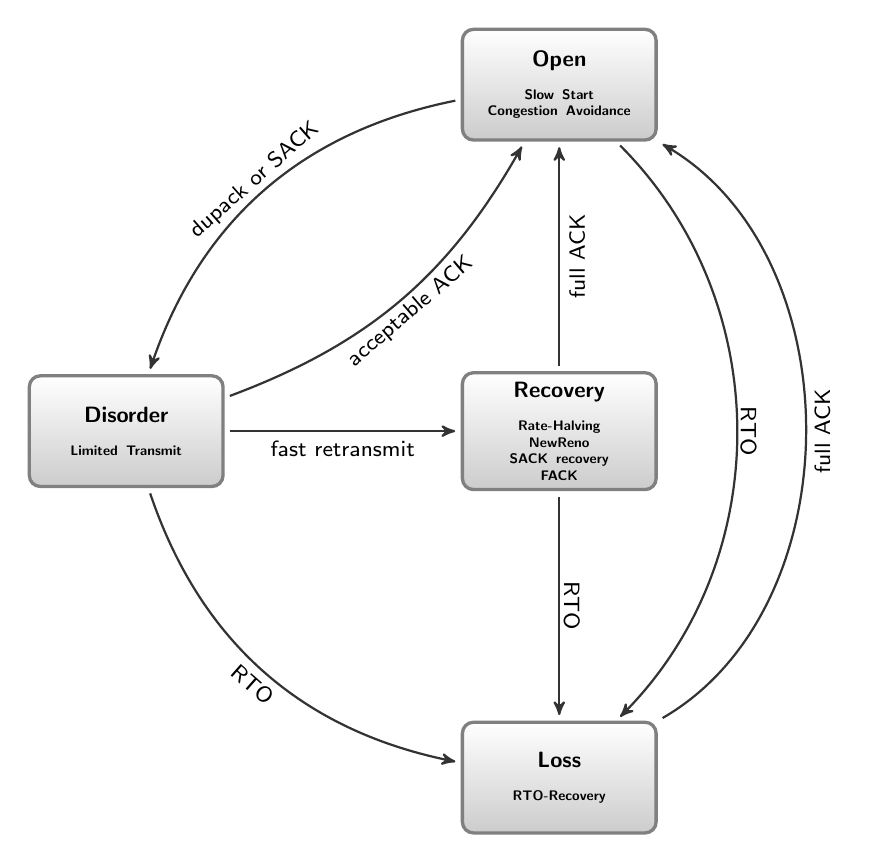
\begin{tikzpicture}[scale=1.1]
    \tikzstyle{preEdge} = [
            shorten <=2pt
    ];
    \tikzstyle{infEdge} = [
            draw=black!80,
            thick
    ];
    \tikzstyle{sufEdge} = [
            shorten >=2pt,
            >=stealth'
    ];
    \tikzstyle{Edge} = [
            preEdge,
            infEdge,
            sufEdge
    ];
    \tikzstyle{EdgeLabel} = [
            midway,
            sloped,
            above=-0.3em,
            font={\sffamily\tiny}
    ];
    \tikzstyle{EdgeLabelBelow} = [
            EdgeLabel,
            font={\sffamily\footnotesize},
            above=-1em,
    ];
    \tikzstyle{EdgeLabelAbove} = [
            EdgeLabel,
            font={\sffamily\footnotesize},
            above=0.1em,
    ];
    \tikzstyle{State} = [
            draw=black!50!black!50,
            top color=white,
            bottom color=black!50!black!20,
            very thick,
            rectangle,
            rounded corners,
            minimum height=4em,
            minimum width=7em,
            text width=5.7em,
            shape=rectangle,
            text centered,
            font={\sffamily\bfseries\footnotesize}
    ];
    
    \node[State, name=Open]     at (0,4) {Open\par\medskip\par{\tiny Slow Start\par Congestion Avoidance\par}};
    \node[State, name=Disorder] at (-5,0){Disorder\par\medskip\par{\tiny Limited Transmit\par}};
    \node[State, name=Recovery] at (0,0) {Recovery\par\medskip\par{\tiny Rate-Halving\par NewReno\par SACK recovery\par FACK\par}};
    \node[State, name=Loss]     at (0,-4){Loss\par\medskip\par{\tiny RTO-Recovery\par}};
    
    \path (Open)     edge [Edge,->,bend right]    node[EdgeLabelAbove] {dupack or SACK} (Disorder)
          (Open)     edge [Edge,->,bend left=45]  node[EdgeLabelAbove] {RTO}            (Loss)
          (Disorder) edge [Edge,->,bend right]    node[EdgeLabelBelow] {RTO}            (Loss)
          (Disorder) edge [Edge,->,bend right=20] node[EdgeLabelBelow] {acceptable ACK} (Open)
          (Disorder) edge [Edge,->,]              node[EdgeLabelBelow] {fast retransmit}(Recovery)
          (Recovery) edge [Edge,->,]              node[EdgeLabelAbove] {RTO}            (Loss)
          (Recovery) edge [Edge,->,]              node[EdgeLabelBelow] {full ACK}       (Open)
          (Loss)     edge [Edge,->,bend right=60] node[EdgeLabelBelow] {full ACK}       (Open);
    \end{tikzpicture}
    \caption{Schöner Graph mit TikZ}
    \label{fig:tikz-graph}
  \end{center}
\end{figure}
